Une maison est constituée d'un parallélépipède rectangle $ABCDEFGH$ surmonté d'un prisme $EFIHGJ$ dont une base est le triangle $EIF$ isocèle en $I$.

Cette maison est représentée ci-dessous.

\begin{center}
	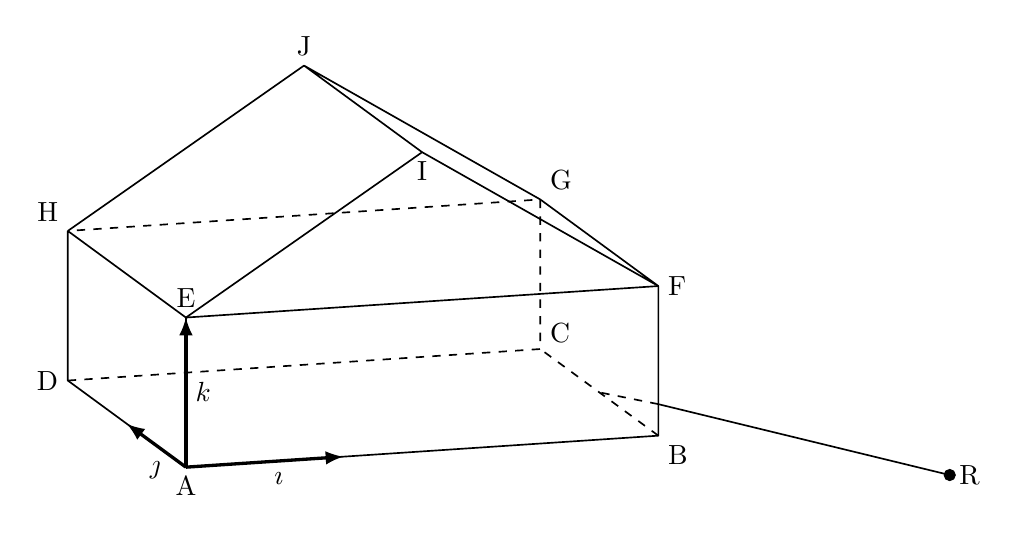
\begin{tikzpicture}[line join=bevel]
		\draw[semithick] (0.4,3.4)--(0.4,1.5)--(1.9,0.4)--(1.9,2.3)--cycle;%HDAE
		\draw[semithick] (1.9,0.4)--(7.9,0.8)--(7.9,2.7)--(1.9,2.3);%ABFE
		\draw[semithick,dashed] (0.4,1.5)--(6.4,1.9)--(6.4,3.8)--(0.4,3.4);%DCGH
		\draw[semithick,dashed] (7.9,0.8)--(6.4,1.9);%BC
		\draw[semithick] (7.9,2.7)--(6.4,3.8)--(3.4,5.5)--(4.9,4.4)--cycle;%FGJI
		\draw[semithick] (4.9,4.4)--(1.9,2.3);%IE
		\draw[semithick] (3.4,5.5)--(0.4,3.4);%JH
		\draw[very thick,->,>=latex] (1.9,0.4)--(3.9,0.533);
		\draw[very thick,->,>=latex] (1.9,0.4)--(1.15,0.95);
		\draw[very thick,->,>=latex] (1.9,0.4)--(1.9,2.3);
		\draw[semithick] (11.6,0.3)--(7.9,1.2);
		\draw[semithick,dashed] (7.9,1.2)--(7.15,1.35);
		%points
		\draw (1.9,0.4) node[below] {A} ;
		\draw (7.9,0.8) node[below right] {B} ;
		\draw (6.4,2.1) node[right] {C} ;
		\draw (0.4,1.5) node[left] {D} ;
		\draw (1.9,2.3) node[above] {E} ;
		\draw (7.9,2.7) node[right] {F} ;
		\draw (6.4,3.8) node[above right] {G} ;
		\draw (0.4,3.4) node[above left] {H} ;
		\draw (4.9,4.4) node[below] {I} ;
		\draw (3.4,5.5) node[above] {J} ;
		\filldraw (11.6,0.3) circle[radius=2pt] node[right] {R} ;
		\draw (1.7,0.6) node[below left] {$\vect{\jmath}$} ;
		\draw (2.9,0.45) node[below right] {$\vect{\imath}$} ;
		\draw (1.9,1.35) node[right] {$\vect{k}$} ;
	\end{tikzpicture}
\end{center}

On a $AB=3$, $AD=2$ et  $AE=1$. On définit les vecteurs $\vect{\imath}= \dfrac13\vect{\text{AB}}$, $\vect{\jmath}= \dfrac12\vect{\text{AD}}$ et $\vect{k} = \vect{\text{AE}}$.

\smallskip

On munit ainsi l'espace du repère orthonormé $\left(A;\vect{\imath},\,\vect{\jmath},\,\vect{k}\right)$.

\begin{enumerate}
	\item Donner les coordonnées du point $G$.
	\item Le vecteur $\vect{n}$ de coordonnées $(2;0;-3)$ est vecteur normal au plan $(EHI)$.
	
	Déterminer une équation cartésienne du plan $(EHI)$.
	\item Déterminer les coordonnées du point $I$.
	\item Déterminer une mesure au degré près de l'angle $\widehat{EIF}$.
	\item Afin de raccorder la maison au réseau électrique, on souhaite creuser une tranchée rectiligne depuis un relais électrique situé en contrebas de la maison.
	
	Le relais est représenté par le point R de coordonnées $(6;-3;-1)$.
	
	La tranchée est assimilée à un segment d'une droite $\Delta$ passant par $R$ et dirigée par le vecteur $\vect{n}$ de coordonnées $(-3;4;1)$. On souhaite vérifier que la tranchée atteindra la maison au niveau de l'arête $[BC]$.
	\begin{enumerate}
		\item Donner une représentation paramétrique de la droite $\Delta$.
		\item On admet qu'une équation du plan $(BFG)$ est $x = 3$.
		
		Soit $K$ le point d'intersection de la droite $\Delta$ avec le plan $(BFG)$.
		
		Déterminer les coordonnées du point $K$.
		\item Le point K appartient-il bien à l'arête $[BC]$ ?
	\end{enumerate}
\end{enumerate}

